\section{Enabling Algorithm-Based Fault Tolerance in MPI}
\label{sect:ompi}

\subsection{The Checkpoint-on-Failure Protocol}

In this paper, we advocate that an extremely efficient form of fault tolerance
can be implemented, strictly based on the MPI standard, for applications capable
of taking advantage of forward recovery. \abft methods are an example of forward
recovery algorithms, capable of restoring missing data from redundant information
located on other processes.  This forward recovery step requires communication
between processes, and we acknowledge that, in light of the current standard,
requiring the MPI implementation to maintain service after failures is too
demanding. However, a high-quality MPI library should at least allow the application to regain control following a process failure. We note
that this control gives the application the opportunity to save its state and
exit gracefully, rather than the usual behavior of being aborted by the MPI
implementation.

\begin{algorithm}
\caption{The Checkpoint-on-Failure Protocol}
\label{alg:on-demand-alg}\label{fig:idea}
\centering
\begin{minipage}[b]{.55\linewidth}
	\begin{enumerate}\sffamily\small
		\item MPI returns an error on surviving processes 
		\item Surviving processes checkpoint
		\item Surviving processes exit
		\item A new MPI application is started
		\item Processes load from checkpoint (if any)
		\item Processes enter \abft dataset recovery
		\item Application resumes
	\end{enumerate}
\end{minipage}
\hfill
\begin{minipage}[b]{.39\linewidth}
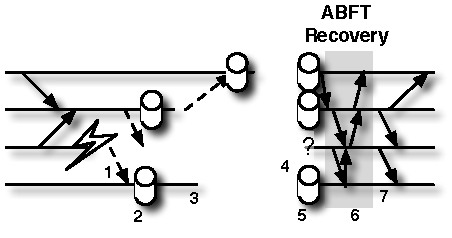
\includegraphics[width=\linewidth]{figures/idea.pdf}
%\caption{Failure recovery execution diagram of On-Demand Checkpointing\label{fig:idea}}
\end{minipage}
\end{algorithm}

Based on these observations, we propose a new approach for supporting
\abft applications, called Checkpoint-on-Failure (\cof).
Algorithm~\ref{alg:on-demand-alg} presents the steps involved in the
\cof method. In the associated explanatory figure, horizontal lines
represent the execution of processes in two successive MPI applications.
When a failure eliminates a process, other processes are notified and
regain control from ongoing MPI calls (1). Surviving processes assume
the MPI library is dysfunctional and do not further call MPI operations
(in particular, they do not yet undergo \abft recovery). Instead, they
checkpoint their current state independently and abort (2, 3). When
all processes exited, the job is usually terminated, but the user (or a
managing script, batch scheduler, runtime support system, etc.) can
launch a new MPI application (4), which reloads processes from
checkpoint (5). In the new application, the MPI library is functional
and communications possible; the \abft recovery procedure is called to
restore the data of the process(es) that could not be restarted from
checkpoint (6). When the global state has been repaired by the \abft
procedure, the application is ready to resume normal execution.

%AURELIEN: true enough, but I need to  cut lines. 
%If another failure hits the system during the recovery, the local states
%are not updated, and the relaunch starts from the beginning. If another
%failure hits the system after the \abft recovery, the same procedure is
%followed to handle it.

Compared to periodic checkpointing, in \cof, a process
pays the cost of creating a checkpoint only when a failure, or multiple simultaneous 
failures have happened,
hence an optimal number of checkpoints during the run (and no checkpoint
overhead on failure-free executions). Moreover, in periodic checkpointing,
a process is protected only when its checkpoint is stored on safe,
remote storage, while in \cof, local checkpoints are
sufficient: the forward recovery algorithm reconstructs datasets of
processes which cannot restart from checkpoint. 
Of course, \cof also exhibits the same overhead as the standard \abft approach: the
application might need to do extra computation, even in the absence of
failures, to maintain internal redundancy (whose degree varies with the 
maximum number of simultaneous failures) used to recover data damaged
by failures. However, \abft techniques often demonstrate excellent
scalability; for example, the overhead on failure-free execution of the
\abft QR operation (used as an example in Section~\ref{sec:ftla}) is inversely
proportional to the number of processes.

\subsection{MPI Requirements for Checkpoint-on-Failure}\label{sec:interface}

\paragraph*{Returning Control over Failures:} In most MPI
implementations, MPI\_ERRORS\_ABORT is the default (and often, only
functional) error handler. However, the MPI standard also defines the
MPI\_ERRORS\_RETURN handler. To support \cof, the MPI
library should never deadlock because of failures, but invoke the error handler, at least on
processes doing direct communications with the failed process. The
handler takes care of cleaning up at the library level and returns
control to the application.

\paragraph*{Termination After Checkpoint:} A process that detects a
failure ceases to use MPI. It only checkpoints on some storage and
exits without calling MPI\_Finalize. Exiting without calling
MPI\_Finalize is an error from the MPI perspective, hence the failure
cascades and MPI eventually returns with a failure notification on every process, which triggers their own checkpoint procedure and termination.

\subsection{\ompi Implementation\label{sec:mpi}}

\ompi is an MPI 2.2 implementation architected such that it contains two
main levels, the runtime (ORTE) and the MPI library (OMPI). As with most
MPI library implementations, the default behavior of \ompi is to abort
after a process failure. This policy was implemented in the runtime
system, preventing any kind of decision from the MPI layer or the
user-level. The major change requested by the \cof protocol was to make the
runtime system resilient, and leave the decision in case of failure to
the MPI library policy, and ultimately to the user application.

\paragraph*{Failure Resilient Runtime:} The ORTE runtime layer provides
an out-of-band communication mechanism (OOB) that relays messages based
on a routing policy. Node failures not only impact the MPI
communications, but also disrupt routing at the OOB level. The
default routing policy in the Open MPI runtime has been amended to allow
for self-healing behaviors; this effort is not entirely 
necessary, but it avoids the significant downtime imposed by a complete 
redeployment of the parallel job with resubmission in queues. The 
underlying OOB topology is automatically updated to route around failed processes. In some routing topologies,
such as a star, this is a trivial operation and only requires excluding
the failed process from the routing tables. For more elaborate
topologies, such as a binomial tree, the healing operation involves
computing the closest neighbors in the direction of the failed process
and reconnecting the topology through them. The repaired topology is
not rebalanced, resulting in degraded performance but complete
functionality after failures. Although in-flight messages that were
currently ``hopping'' through the failed processes are lost, other
in-flight messages are safely routed on the repaired topology. Thanks to self-healing topologies, the runtime remains responsive, even when MPI processes leave. 
%This persistent
%runtime avoids losing the batch scheduler reservation and eliminates the cost
%of redeploying the runtime infrastructure.
% It also remains available for spawning replacement MPI processes, and to
% access locally stored checkpoints.

\paragraph*{Failure Notification:} The runtime has been augmented with a
failure detection service. To track the status of the failures, an
incarnation number has been included in the process names. Following a
failure, the name of the failed process (including the incarnation
number) is broadcasted over the OOB topology. By including this
incarnation number, we can identify transient process failures, prevent
duplicate detections, and track message status. ORTE processes monitor
the health of their neighbors in the OOB routing topology. Detection of
other processes rely on a failure resilient broadcast that overlays on
the OOB topology. This algorithm has a low probability of creating a
bi-partition of the routing topology, hence ensuring a high accuracy of
the failure detector. However, the underlying OOB routing algorithm has
a significant influence on failure detection and propagation time, as
the experiments will show. On each node, the ORTE runtime layer forwards
failure notifications to the MPI layer, which has been modified to
invoke the appropriate MPI error handler.
%(MPI\_ERR\_RETURNS, or a custom error handler). MPI calls are interrupted and
%the application regains control. The MPI library purges internal queues and
%state, to minimize the size of checkpoint.
